\begin{figure}

  \setlength{\unitlength}{\textwidth}
  
 \begin{picture}(1,0.399)(0.01,0.77)
     % % % 90
     \put(0.03,1){\includegraphics[width=0.35\unitlength]{../FnP/gnuplot/vel_time_history_1164.eps}}   
     \put(0.36,1){\includegraphics[width=0.35\unitlength]{../FnP/gnuplot/vel_time_history_10.eps}}
     \put(0.68,1){\includegraphics[width=0.35\unitlength]{../FnP/gnuplot/vel_time_history_5.eps}}
         
     \put(0.03,0.82){\includegraphics[width=0.35\unitlength]{../FnP/gnuplot/dis_time_history_1164.eps}}   
     \put(0.36,0.82){\includegraphics[width=0.35\unitlength]{../FnP/gnuplot/dis_time_history_10.eps}}
     \put(0.68,0.82){\includegraphics[width=0.35\unitlength]{../FnP/gnuplot/dis_time_history_5.eps}}
     
 
     
     \put(0.55,0.79){$\displaystyle{\frac{tU}{D}}$}
     \put(0.2,0.79){$\displaystyle{\frac{tU}{D}}$}
     \put(0.85,0.79){$\displaystyle{\frac{tU}{D}}$}
     
      \put(0.02,1.07){$\displaystyle\frac{V}{D}$}
     \put(0.02,0.9){$\displaystyle\frac{A}{D}$}
 
     
     \put(0.08,0.9997){(a)}    
     \put(0.4,0.9997){(b)}    
     \put(0.72,0.9997){(c)}
     \put(0.08,0.8){(d)}    
     \put(0.4,0.8){(e)}    
     \put(0.72,0.8){(f)}
     
    
   \end{picture}


  \caption{Time histories of velocity. Data presented at \reynoldsnumber=22300, $m^*=10$ and $\frac{c}{\rho\mathcal{A}U}=9.3\times10^{-1}$ at three different reduced velocities: (a) $\ustar=75$, (b) $\ustar=175$ and (a) $\ustar=375$. As the mass ratio decreases the signal tend to transform from a sinusoidal towards a square signal due to the reduction in inertia.}
  
  \label{time_history_mstar}
\end{figure}
